\chapter{Experiments}\label{ch:experiments}

A number of experiments have been done in order to find the differences in effectiveness between different architectures. For all of these experiments, only 0.1\% of the data set has been used. Due to the number of experiments, a higher percentage would take significantly longer. Because this number is so small, it is not a perfect representation of the data set. However, while only 0.1\% of users (13 users) are in this data set, these users together represent a total of 6117530 actions (around 0.6\% of the total data set), meaning these users represent a higher amount of the data set than they themselves make up. Even though these experiments are not done on 100\% of the data set, significant differences in effectiveness are likely to persist in bigger data sets.

The base architecture that all the experiments are compared to is the architecture described in Chapter~\ref{ch:methods}. To summarize, 2 layers of standard LSTMs with a single Dense layer. All using a batch size of 32 and 25 epochs.

\section{Batch Size}
Experiments regarding increasing or decreasing the batch size were done. Changing the batch sizes to 64 and 16 respectively. No significant differences were observed. The amount of anomalies found were the same between all configurations in this experiment. The IQR values were also all the same. From this it can be concluded that changing the batch size to be bigger or smaller has little effect (at least in this portion of the data set and with these numbers). Seeing as increasing the batch size significantly increases performance, increasing it would be an easy way to speed up the system. However, increasing the batch size by too much has been shown to reduce the effectiveness of neural networks.


\begin{figure}
	\begin{center}
		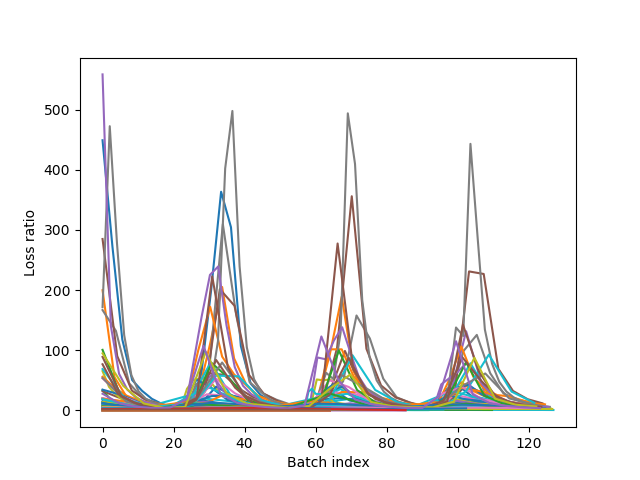
\includegraphics[scale=0.7]{experiments/epochs/25-epochs.png}
	\end{center}
	\caption{The ratio between the highest loss event and the average loss of a batch, using 25 epochs.~\label{fig:25-epochs}}
\end{figure}


\begin{figure}
	\begin{center}
		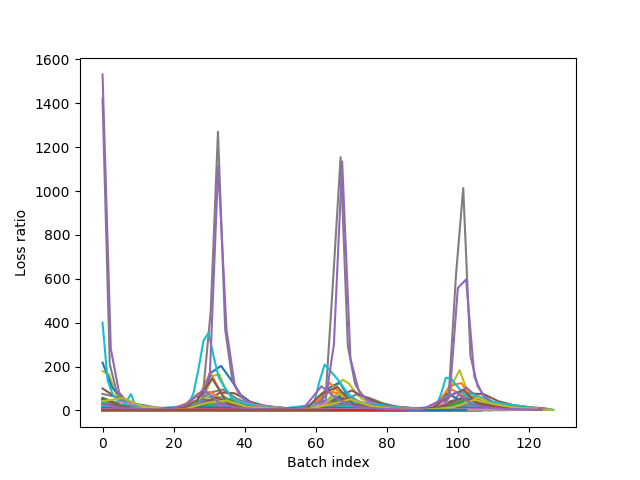
\includegraphics[scale=0.7]{experiments/epochs/15-epochs}
	\end{center}
	\caption{The ratio between the highest loss event and the average loss of a batch, using 15 epochs.~\label{fig:15-epochs}}
\end{figure}


\begin{figure}
	\begin{center}
		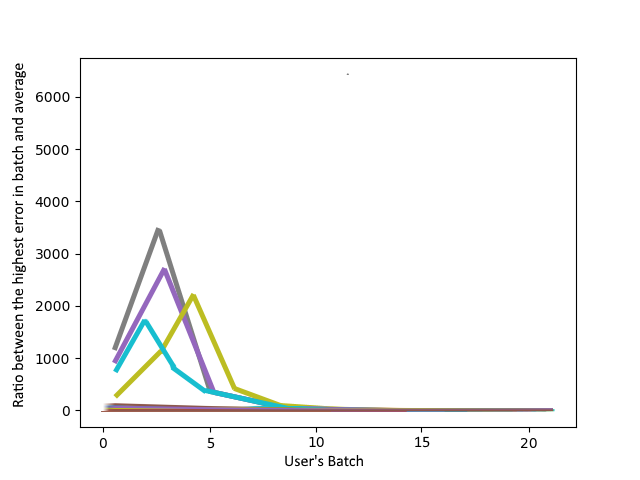
\includegraphics[scale=0.7]{experiments/epochs/8-epochs}
	\end{center}
	\caption{The ratio between the highest loss event and the average loss of a batch, using 8 epochs.~\label{fig:8-epochs}}
\end{figure}

\section{Epochs}
Changing the epoch sizes to 15 and 40 has also shown little difference in the results with the current setup. However, some experiments with a number of different epoch sizes have been done on a set of users with a very low amount of actions (~1500 per user). The architecture was also different, having no dropout rate on the LSTM layers. This showed some significant differences in the results. Figures~\ref{fig:25-epochs},~\ref{fig:15-epochs} and~\ref{fig:8-epochs} show significant differences between the highest loss value and the average loss value of a batch. This is likely because epoch sizes that low tend to have a big effect when given little training data. The effect of a high epoch size is to essentially train multiple times on the same data. When there is a lot of data available, this is not necessary, instead causing the network to overfit on the input data it has. The differences between these two test scenarios can likely be explained by the first scenario having a dropout rate, significantly reducing the amount of overfitting a higher epoch size brings, and also having a lot more input data, making a lower epoch size have less effect as well.

\section{Shared weights}
The possibility of using one neural network for all users was explored. However, this introduced some problems. One of these is that the total amount of actions for all users was not the same. This leads to the system weighing the actions of high-volume users heavier than those of low-volume users, leading to an unfair representation of the \enquote{average} user's behavior. Another problem was that performance was significantly worse. Parallelization can not be applied as the single network has to be kept in memory for the entire process. The network also gravitates towards learning the behavior of \enquote{average} users. It will try to find a middle ground in the behavior of different types of users (sysadmins vs users that rarely log in), never really learning a single user's behavior well enough to find slight deviations. It will then accept users such as sysadmins having a high error value as normal, which could be very dangerous if such an account gets compromised.

\begin{figure}
	\begin{center}
		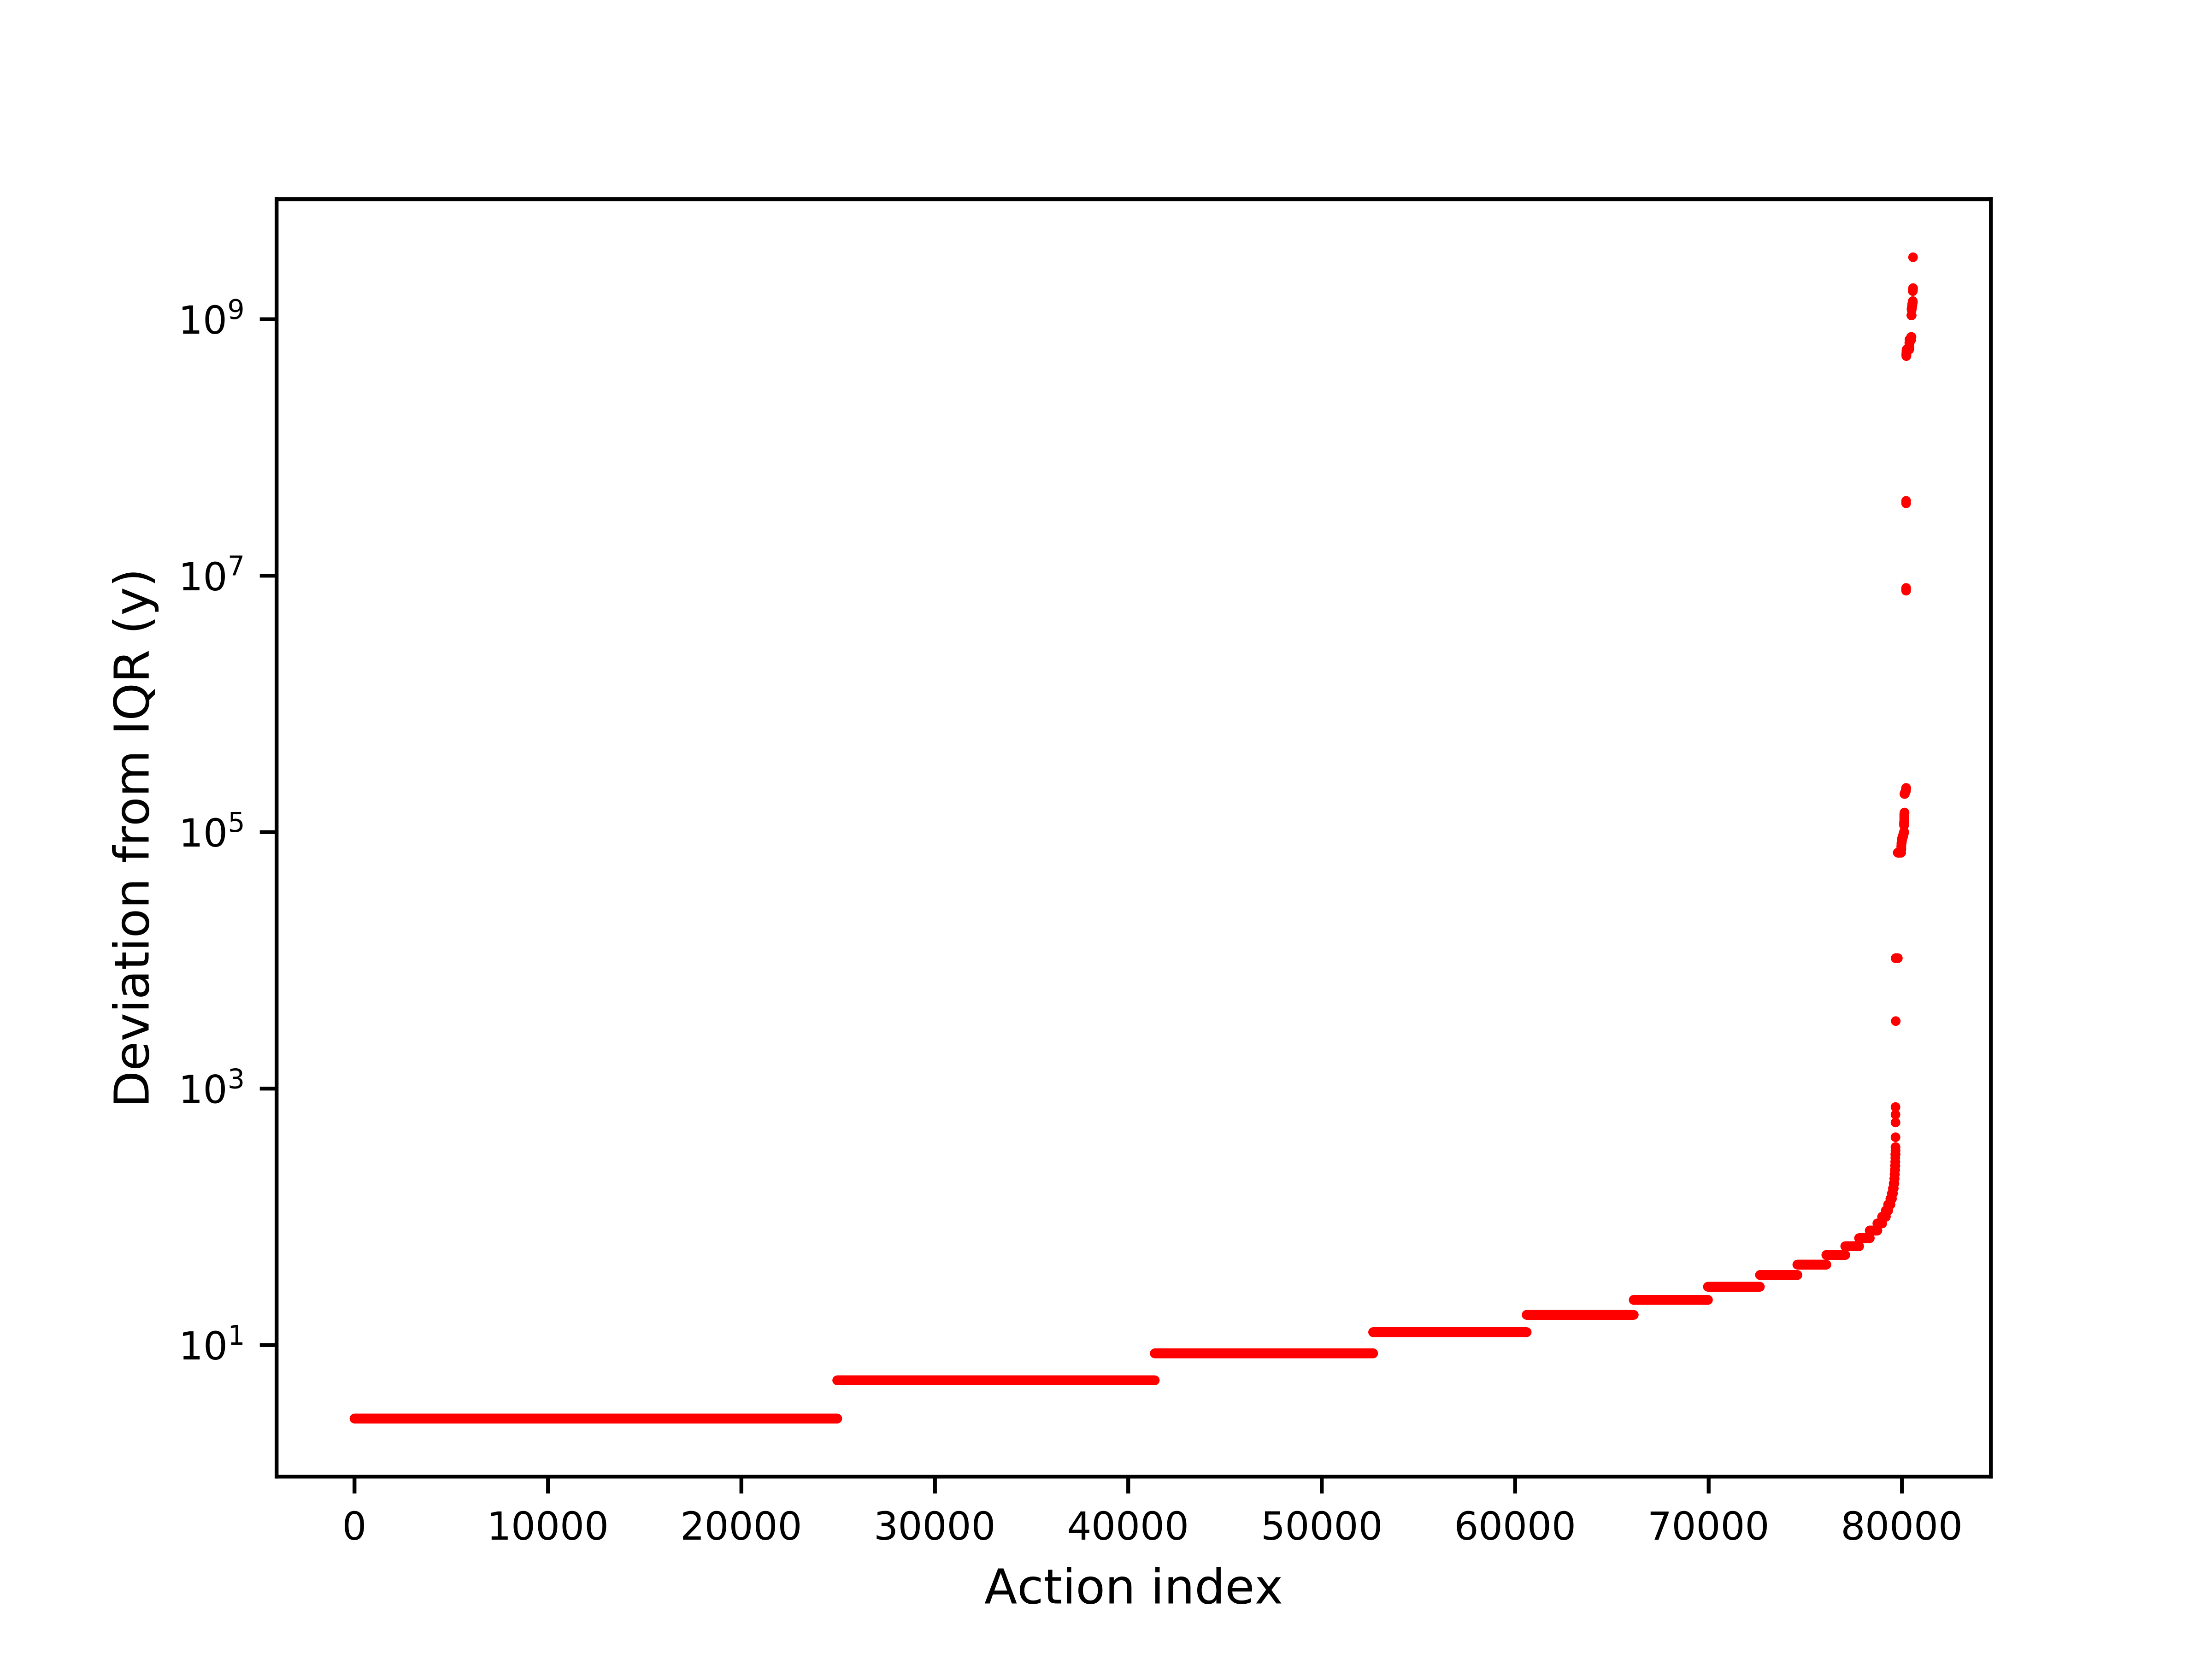
\includegraphics[scale=6.0]{experiments/cell/deviations/gru}
	\end{center}
	\caption{The deviations \(y\) (function ~\ref{eq:y}) of the mean squared errors of all predicted test set feature vectors compared to the actual feature vectors. Using GRU cells.~\label{fig:gru_deviations}}
\end{figure}

\begin{figure}
	\begin{center}
		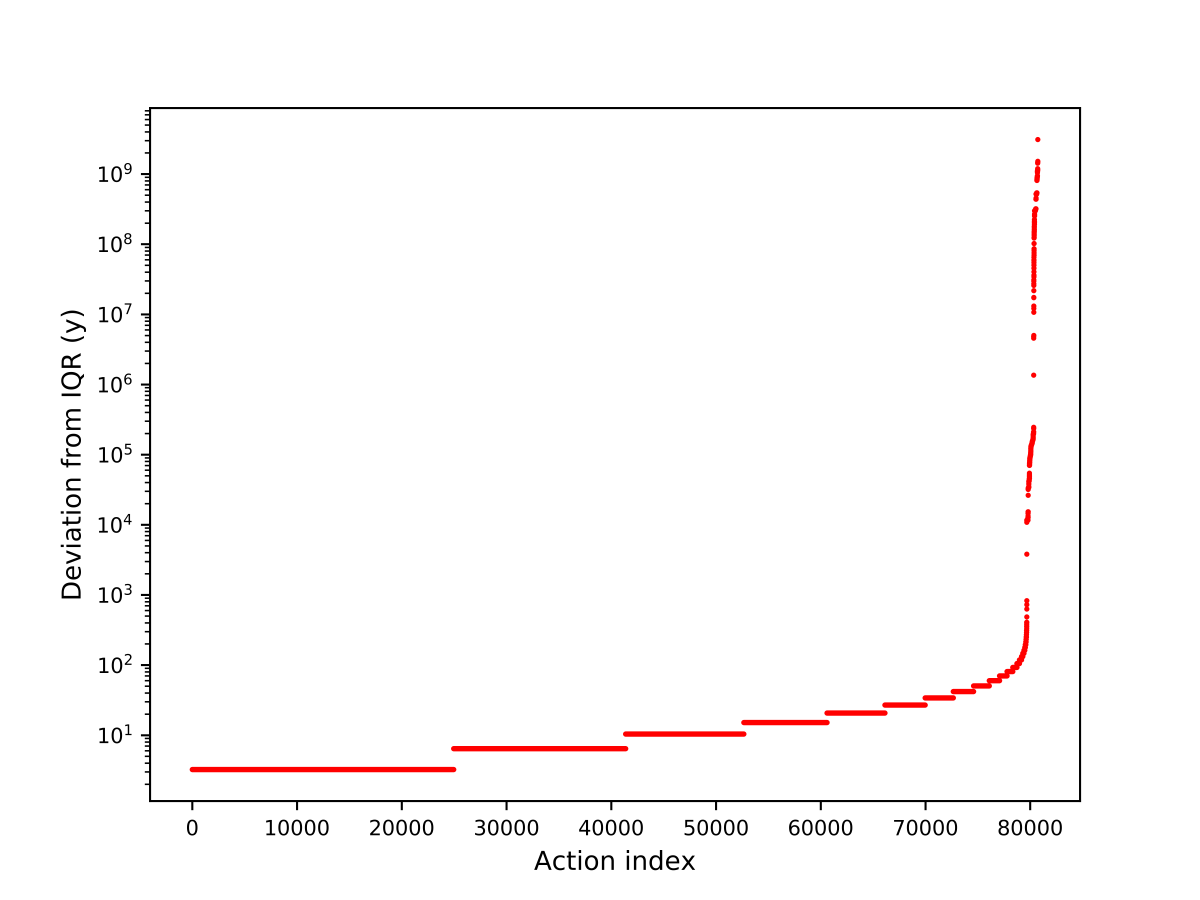
\includegraphics[scale=6.0]{experiments/cell/deviations/lstm}
	\end{center}
	\caption{The deviations \(y\) (function ~\ref{eq:y}) of the mean squared errors of all predicted test set feature vectors compared to the actual feature vectors. Using LSTM cells.~\label{fig:lstm_deviations}}
\end{figure}

\begin{figure}
	\begin{center}
		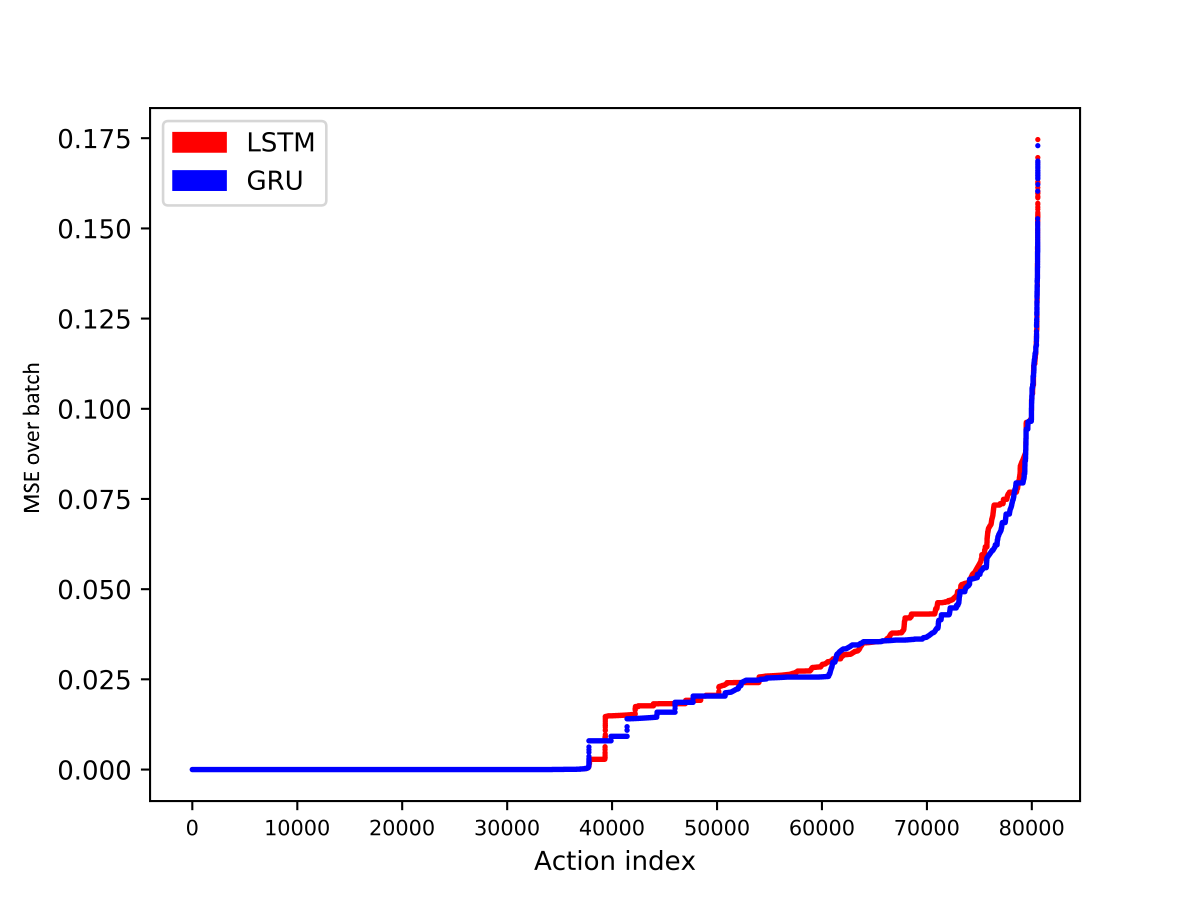
\includegraphics[scale=6.0]{experiments/cell/losses/comparison}
	\end{center}
	\caption{The loss calculated over each batch using the mse.~\label{fig:gru_rnn_losses}}
\end{figure}

\section{GRU cell}
Using a different RNN cell has also been explored. One of these different RNN cells is the GRU cell, introduced in~\cite{cho2014learning}. The differences between an architecture using a LSTM cells and an architecture using GRU cells were slight. As~\cite{chung2014empirical} showed, the performance of GRU cells and LSTM cells are very similar when it came to the area of polyphonic music modeling and speech signal modeling. As such, it is likely that their performance on the area of cyber-security is also similar. Figures~\ref{fig:gru_deviations} and~\ref{fig:lstm_deviations} show that the architecture using LSTM cells has more events with a high deviation than the architecture using GRU cells. This can point to it detecting more actual anomalies, or it labeling non-anomalous actions as anomalies. Because the data set is unlabeled there is unfortunately no way to find out. Figures~\ref{fig:gru_rnn_losses} again shows that the architecture using LSTMs has a higher loss value for most batches, also peaking higher. The LSTM architecture also flagged 0.7\% more events as anomalies. Again conclusions can not be drawn regarding which result is more effective but it can be seen that they do differ somewhat.

\begin{figure}
	\begin{center}
		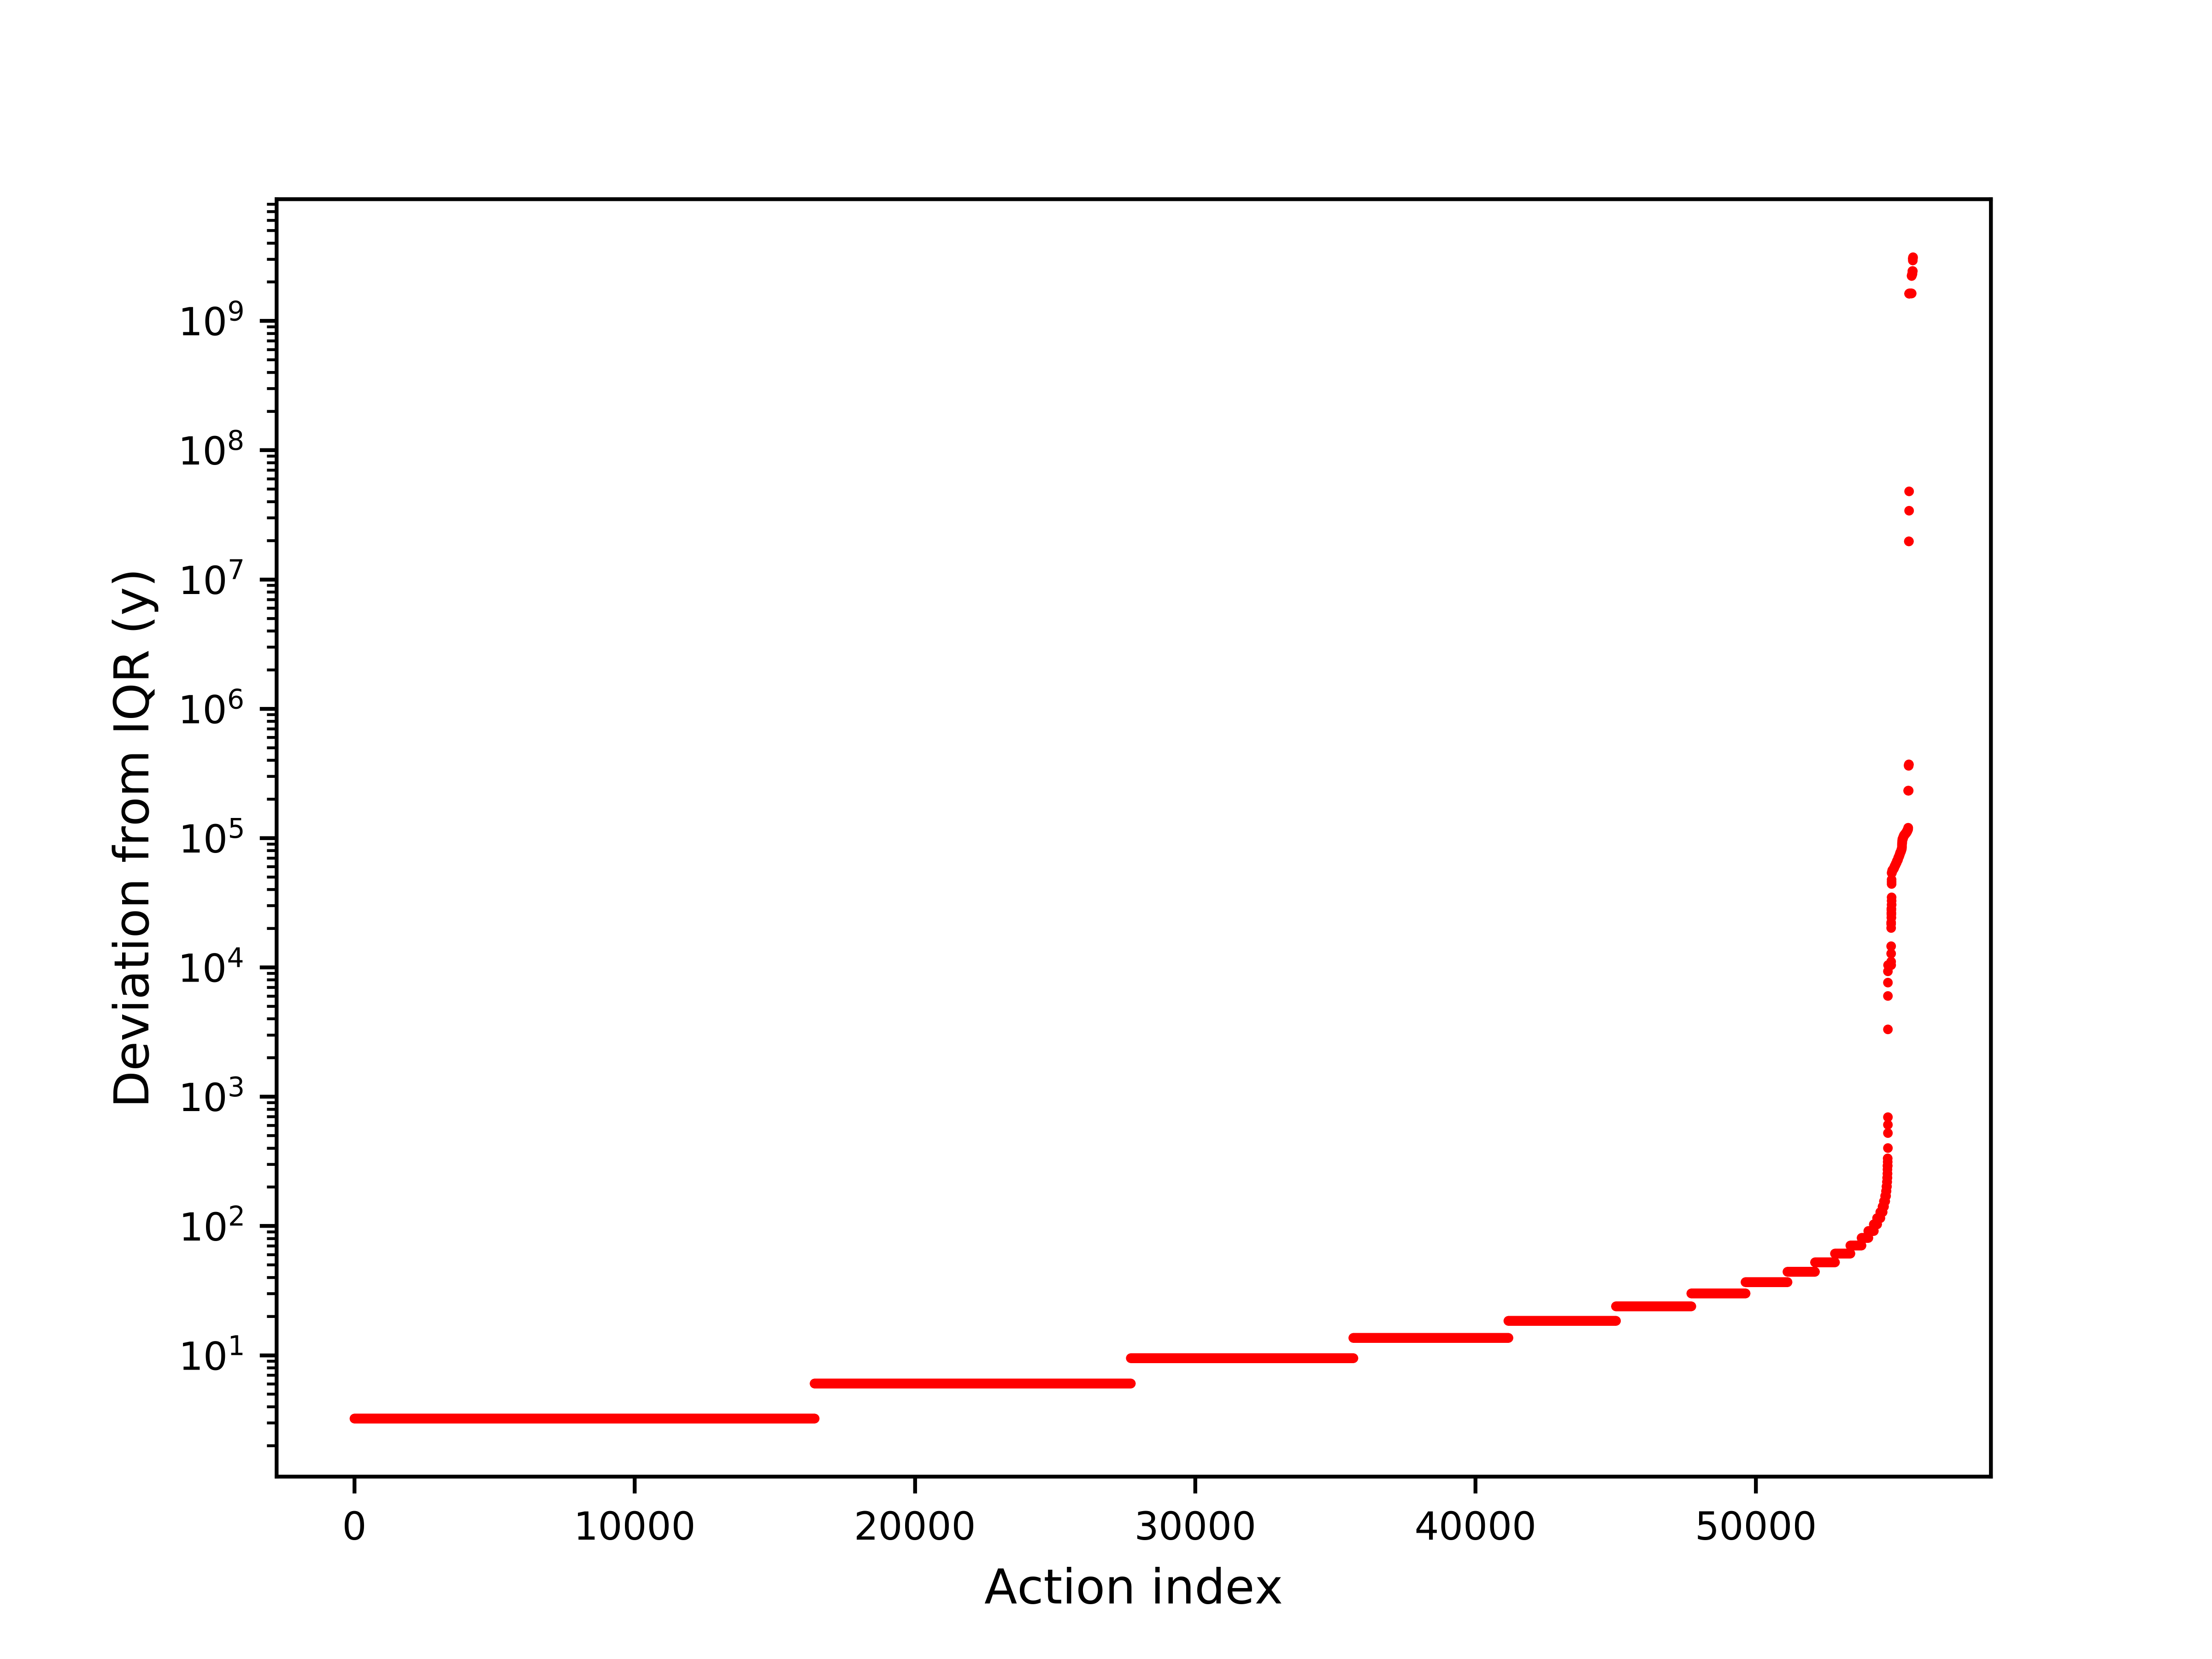
\includegraphics[scale=6.0]{experiments/cell/deviations/rnn}
	\end{center}
	\caption{The deviations \(y\) (function ~\ref{eq:y}) of the mean squared errors of all predicted test set feature vectors compared to the actual feature vectors. Using RNN cells.~\label{fig:rnn_deviations}}
\end{figure}

\section{RNN cell}
Using standard RNN cells instead of an LSTM cells showed a significant difference. Just as with the GRU cells, the RNN cells have significantly lower losses, as can be seen when comparing figures~\ref{fig:lstm_deviations} and~\ref{fig:rnn_deviations}. The RNN cells also flagged less events as anomalous, flagging 21\% less as such. Once again no clear conclusion can be drawn from which one is more effective, however, LSTMs have been shown to be superior to regular RNNs in many fields, suggesting that this may also be a case of the LSTM cells outperforming the RNN cells at finding anomalies.